%\documentclass[12pt]{beamer}
\documentclass{beamer}

\usepackage{amssymb,amsmath,mathtext}
\usepackage{indentfirst,amsfonts}
\usepackage{makecell,multirow,longtable}
\usepackage{verbatim}
\usepackage {graphicx}
\usepackage{tabularx}
\usepackage{makecell}

\usepackage[russian]{babel}
\usepackage[T2A]{fontenc}
\usepackage[utf8]{inputenc}
\usepackage {paratype}

\PassOptionsToPackage{unicode}{hyperref}
\PassOptionsToPackage{naturalnames}{hyperref}

\setbeamertemplate{navigation symbols}{}

\usetheme{Madrid}
%\usetheme{Boadilla}
%\usetheme{Warsaw}


\beamersetuncovermixins{\opaqueness<1>{30}}{\opaqueness<2->{25}}

\deftranslation[to=russian]{example}{пример}
\deftranslation[to=russian]{Example}{Пример}

\makeatletter
\setbeamertemplate{footline}
{
  \leavevmode%
  \hbox{%
  \begin{beamercolorbox}[wd=.333333\paperwidth,ht=2.25ex,dp=1ex,center]{author in head/foot}%
  \end{beamercolorbox}%
  \begin{beamercolorbox}[wd=.333333\paperwidth,ht=2.25ex,dp=1ex,center]{title in head/foot}%
  \end{beamercolorbox}%
  \begin{beamercolorbox}[wd=.333333\paperwidth,ht=2.25ex,dp=1ex,right]{date in head/foot}%
    \usebeamerfont{date in head/foot}\insertshortdate{}\hspace*{2em}
    \insertframenumber{} / \inserttotalframenumber\hspace*{2ex} 
  \end{beamercolorbox}}%
  \vskip0pt%
}
\makeatother

\begin{document}
\title[Алгоритмы извлечения полей]{Алгоритмы и программная система извлечения информационных полей из слабоструктурированных документов}
\author{Н. С. Линецкий\\
\ \\
Направление подготовки:\\
Фундаментальная информатика и информационные технологии\\
\ \\
Руководитель:\\
доцент, к.т.н. М. Г. Адигеев}
\date{Ростов-на-Дону, 2017} 
\institute{Южный Федеральный Университет\\
Институт математики, механики и компьютерных наук имени И. И. Воровича}

{
	\setbeamertemplate{footline}{} 
	\begin{frame}
		\titlepage
	\end{frame}
}

\begin{frame}{Содержание}
\tableofcontents
\end{frame}

\section{Постановка задачи}
\begin{frame}
\frametitle{Постановка задачи}
\begin{itemize}
	\item Изучение существующих алгоритмов и программных решений для извлечения информации из текстов на естественном языке
	\item Разработка системы для извлечения реквизитов с учетом специфики слабоструктурированных документов
	\item Обеспечение возможности конфигурировать систему извне путем задания правил, описывающих шаблоны полей
\end{itemize}
\end{frame}

\section{Введение}
\begin{frame}
\frametitle{Введение}
\begin{itemize}
	\item Необходимость автоматизации процесса обработки электронных документов
	\item Существующие решения не учитывают специфику работы со слабоструктурированными текстами
\end{itemize}
\begin{example}
Гражданин Иванов Иван Иванович, именуемый в дальнейшем <<Наймодатель>>, с одной стороны, и гражданин Петров Петр Петрович, именуемый в дальнейшем <<Наниматель>>, с другой стороны, именуемые в дальнейшем <<Стороны>>, заключили настоящий договор, в дальнейшем <<Договор>>, о нижеследующем:
\end{example}
\end{frame}

\begin{frame}
\frametitle{Концепция решения: Томита-парсер}
\begin{itemize}
	\item Программа для извлечени фактов из текстов на естественном языке
	\item Разработана в Яндексе, исходные коды открыты
	\item Реализует алгоритм GLR-парсинга
	\item Не имеет средств задания контекста для искомых данных
\end{itemize}
\end{frame}

\section{Концепция решения}
\begin{frame}
\frametitle{Концепция решения: структура}
%Три основных модуля:
%\begin{itemize}
%	\item Разметка входного текста договора
%	\item Анализ входных правил, описывающих шаблоны искомых полей
%	\item Извлечение полей с использованием алгоритма Томиты
%\end{itemize}
\begin{figure}% p означает, что нужно выделить для рисунка
\centering
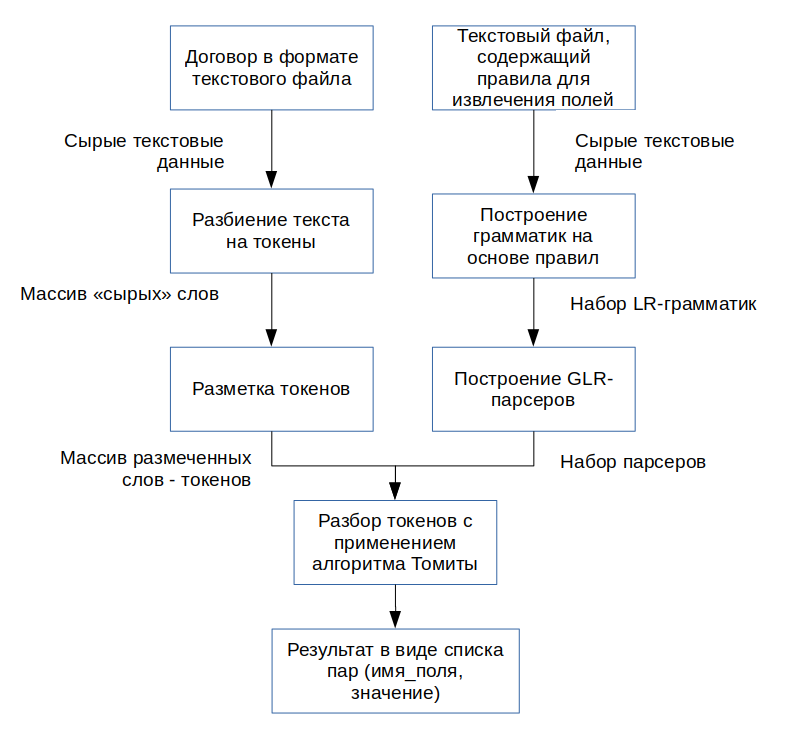
\includegraphics[width=0.7\textwidth]{img/ProjectDiagramPres.png}
\end{figure}
\end{frame}

%\begin{frame}[fragile]
%\frametitle{Концепция решения: алгоритм Томиты}
%\begin{itemize}
%	\item Разработан японским ученым Масару Томитой
%	\item Generalized LR парсер
%	\item Graph Structured Stack: стек разбора с поддержкой операций ветвления и слияния
%\end{itemize}
%\begin{figure}% p означает, что нужно выделить для рисунка
%\centering
%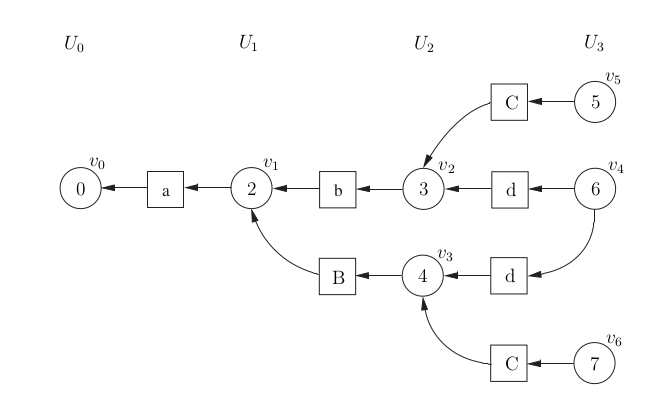
\includegraphics[width=0.7\textwidth]{img/gss-step5.png}
%\end{figure}
%\end{frame}

\section{Реализация}
\begin{frame}[fragile]
\frametitle{Реализация: разметка текста}
\begin{itemize}
	\item Разложение текста на элементарные конструкции - слова
	\item Выделение морфологических и семантических свойств для слов
	\item Морфологический анализатор - pymorphy2:
	\begin{itemize}
		\item Аанализа на основе данных из OpenCorpora
		\item Реализована поддержка разбора несловарных слов
	\end{itemize}
\end{itemize}
\begin{example}[Разбор слова]
Результат разбора слова <<стали>> с помощью pymorphy2:
\begin{enumerate}
	\item Нормальная форма: стать, глагол, прошедшее время, совершенный вид, множественное число, индекс уверенности: 0.78
	\item Нормальная форма: сталь, существительное, женский род, единственное число, индекс уверенности: 0.22
\end{enumerate}
\end{example}
\end{frame}

\begin{frame}[fragile]
\frametitle{Реализация: пользовательские правила}
\begin{itemize}
	\item Две секции: секция правил и секция команд
	\item Запись правил производится в формате $S = right\_handle_1\ |\ right\_handle_2\ |\ ...\ |\ right\_handle_n$, где $S$ - имя искомого реквизита, $right\_handle_i$ - шаблон, описывающий реквизит
	\item Ограничительные пометки: регистр, число, род и др.
	\item Определен ряд встроенных правил и слов
\end{itemize}
\begin{example}[Запись встроенного правила, описывающего полное имя человека]
\begin{verbatim}
PersonFullName = Surname SecPart;
SecPart = FullRec | ShordRec;
FullRec = name patr;
ShortRec = init init;
Surname = surn | word(upper1);
\end{verbatim}
\end{example}
\end{frame}

\begin{frame}[fragile]
\frametitle{Реализация: пользовательские правила}
\begin{itemize}
	\item В секции команд указываются искомые правила c дополнительными параметрами поиска
	\item Команда Find:\\ 
	$Find\ rule\_name\ [hint\_words]\ [dependencies]\ [alias]$, где\\
	$rule\_name$ - имя искомого правила\\
	$dependencies$ - список правил-зависимостей\\
	$hint\_words$ - контекст\\
	$alias$ - псевдоним правила
\end{itemize}
\begin{example}
Find PersonFullName (hint\_words: "наниматель") as Employer;\\
Find FullDate with deps (left: Town) as AgreementDateValue;
\end{example}
\end{frame}

\begin{frame}
\frametitle{Реализация: извлечение полей}
\begin{itemize}
	\item Построение контекстно-свободной грамматики $G = (\Sigma, N, P, S$)
	\item Построение LR-анализатора
	\item Разбор входного текста с помощью алгоритма Томиты
	\begin{itemize}
		\item GSS формируется по одному уровню за итерацию
		\item Узлы текущего уровня - активные
	\end{itemize}
\end{itemize}
\begin{figure}% p означает, что нужно выделить для рисунка
\centering
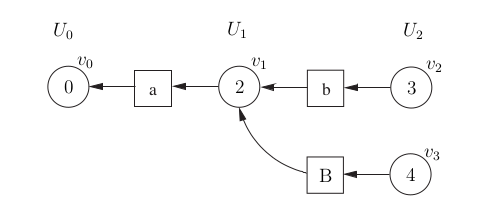
\includegraphics[width=0.7\textwidth]{img/gss-step3.png}
\end{figure}
\end{frame}

\begin{frame}
\frametitle{Реализация: зависимости и контекст}
\begin{itemize}
	\item Зависимости по пространственному признаку: левые, правые, верхние, нижние
	\item Поле считается найденым только тогда, когда найдены все его зависимости
	\item Контекстные слова характеризуют семантику слова: в деловой речи можно выделить весьма ограниченный набор таких слов
	\item Эвристика поиска: $\sum_{n=1}^{N} \frac{1}{|Dist(W,w_n)|}$, где\\
	$N$ - количество найденных контекстных слов\\
	$W = w_1...w_k$ - результат разбора для некоторого правила $S$\\
	$w_n$ - найденное ключевое слово к текущем абзаце
\end{itemize}
\end{frame}

\section{Пример работы}
\begin{frame}[shrink=30]
\frametitle{Пример работы}
\begin{center}
\begin{tabularx}{\textwidth}{| X | X | X |}
\hline
\textbf{Текст договора} & \textbf{Набор правил} & \textbf{Результат} \\ 
\hline
Гражданин Меркулов Сергей Андреевич, именуемый в дальнейшем «Наймодатель», с одной стороны, и гражданин Меркулов Андрей Андреевич, именуемый в дальнейшем «Наниматель», заключили настоящий договор, далее «Договор»,  на следующих условиях: & Find PersonFullName (hint\_words: "наниматель") as Employer; & Иванов Андрей Андреевич \\ 
\hline
1. ПРЕДМЕТ НАСТОЯЩЕГО ДОГОВОРА
1.1. Наймодатель предоставляет Нанимателю помещение, состоящее из трех комнаты, (в трехкомнатной квартире) расположенное по адресу город Ростов-на-Дону, улица Волкова, дом 5, квартира 184 за плату, во временное пользование в целях проживания. & Find Address (hint\_words: "располагаться"\, "находиться"\, "адрес") 
as ApartementAddress; & город Ростов-на-Дону улица Волкова дом 5 \\ \hline
\end{tabularx}
\end{center}
\end{frame}

%\begin{frame}
%\frametitle{Реализация: извлечение полей}
%Этапы итерации:
%\begin{description}
%	\item[Actor] получение все $action$
%	\item[Reducer] выполнение активных сверток
%	\item[Shifter] выполнение активных сдвигов и формирование следующего уровня 
%\end{description}
%\begin{figure}% p означает, что нужно выделить для рисунка
%\centering
%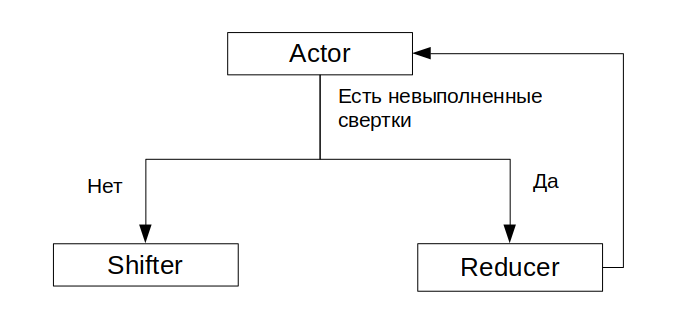
\includegraphics[width=\textwidth]{img/glr-iteration.png}
%\end{figure}
%\end{frame}

\section{Результаты}
\begin{frame}
\frametitle{Результаты}
\begin{itemize}
	\item Изучены существующие алгоритмы и программные решения для извлечения информации из текстов на естественном языке
	\item Разработана система для извлечения реквизитов с учетом специфики слабоструктурированных документов
	\begin{itemize}
		\item Процедура извлечения производится с помощью алгоритма Томиты
		\item В процессе разбора учитываются морфологические и семантические свойства текста
		\item Осуществляется анализ ключевых слов и зависимостей
	\end{itemize}
	\item Обеспечена возможность конфигурировать систему извне путем задания правил, описывающих шаблоны полей
	\begin{itemize}
		\item Реализован декларативный язык описания структуры полей и параметров поиска
	\end{itemize}
\end{itemize}
\end{frame}

\end{document}
